%!TEX TS-program = pdflatex
%!TEX encoding = UTF-8 Unicode

\documentclass[12pt,a4paper,twoside,english, italian]{book}

\usepackage[utf8]{inputenc}
\usepackage{babel}
\usepackage{uniudtesi}
\usepackage{siunitx}
\usepackage[nottoc]{tocbibind}
\usepackage{indentfirst}
\usepackage{emptypage}
\usepackage{algorithm}
\usepackage{algpseudocode}
\usepackage{xcolor}
\graphicspath{{./figure/}}
\usepackage{amsmath,amsfonts,amssymb,amsthm}
\usepackage{latexsym}
\usepackage{listings} 
\newcommand{\N}{\mathbb{N}}
\newcommand{\Z}{\mathbb{Z}}
\newcommand{\Q}{\mathbb{Q}}
\newcommand{\R}{\mathbb{R}}
\newcommand{\Complessi}{\mathbb{C}}
\usepackage{fancyhdr}
\pagestyle{fancy}
\renewcommand{\chaptermark}[1]{\markboth{#1}{}}
\renewcommand{\sectionmark}[1]{\markright{\thesection\ #1}}
\fancyhf{}
\fancyhead[LE,RO]{\bfseries\thepage}
\fancyhead[LO]{\bfseries\rightmark}
\fancyhead[RE]{\bfseries\leftmark}
\renewcommand{\headrulewidth}{0.5pt}
\renewcommand{\footrulewidth}{0pt}
\setlength{\headheight}{14.5pt}

\usepackage[backend=bibtex,style=ieee]{biblatex}
\bibliography{bibliography} 


  \titolo{Compression in time series \\databases}
 \laureando{Umberto D'Ovidio}
  \annoaccademico{2018-2019}
\corsodilaureatriennalein{Tecnologie Web e Multimediali}
  \relatore[Prof.]{Nicola Vitacolonna}
 \begin{document}
\selectlanguage{english}

\frontmatter
\maketitle


\renewcommand{\theequation}{\arabic{equation}}%consigliato per migliorare i numeri di equazione nell'introduzione
\renewcommand{\thesection}{\arabic{section}}%consigliato per migliorare i numeri di equazione nell'introduzione

\tableofcontents

\mainmatter

\renewcommand{\theequation}{\thechapter.\arabic{equation}}%si torna alle formule numerate come da default
\renewcommand{\thesection}{\thechapter.\arabic{section}}%si torna alle sezioni numerate come da default


%!TEX TS-program = pdflatex
%!TEX root = tesi.tex
%!TEX encoding = UTF-8 Unicode


     %%%%%%%%%%%%%%%%%%%%
     %                  %
     %  capitolo1.tex   %
     %                  %
     %%%%%%%%%%%%%%%%%%%%

\chapter{Introduction to Time Series Data}

\section{What is time series data?}
Time series data can be thought of as a series of data points, measuring a certain variable
over time, stored in time order. Time Series datasets most commonly share three
characteristics \cite{AjayKulkarni2018What} :
\begin{itemize}
	\item Data points are almost always stored as a new record
	\item Data typically arrive in time order
	\item Time is the most important feature of time series data and is a key attribute that distinguishes it from other data
\end{itemize}

For example, let us consider the S\&P 500, a stock market index based on the market
capitalization of the largest 500 companies in the USA. We can collect valuable information
during a given time interval. For example, we could be interested in the high, low and closing
price on a daily basis. The dataset is illustrated in Figure~\ref{sp500}.

\begin{figure}
\begin{center}
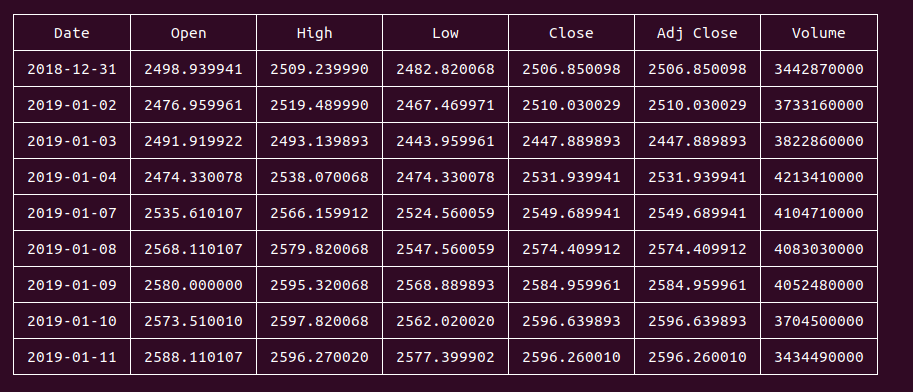
\includegraphics[width=400pt]{sp500}
\caption[sp500]{Time series values for the S\&P 500 aggregated on a daily basis}
\label{sp500}
\end{center}
\end{figure}

The date column is the time index, while the other columns represent measurements of some
specific metrics. This is a typical example of time series data, although not every dataset
containing date/time information is necessarily a time series data set.

The rule of thumb is that with time series data sets changes over time are tracked by creating
new records, rather than updating existing ones. If you have a record with a timestamp, and
whenever something changes in the measurement you create a new record instead of updating the
previous one, then you have a time series dataset.


\section{What is the importance of time series data?}
Time series data is becoming increasingly important in our world, as one can infer from the
growing popularity of time series databases in the period 2017-2019 (Figure~\ref{tspopularity}).

\begin{figure}
\begin{center}
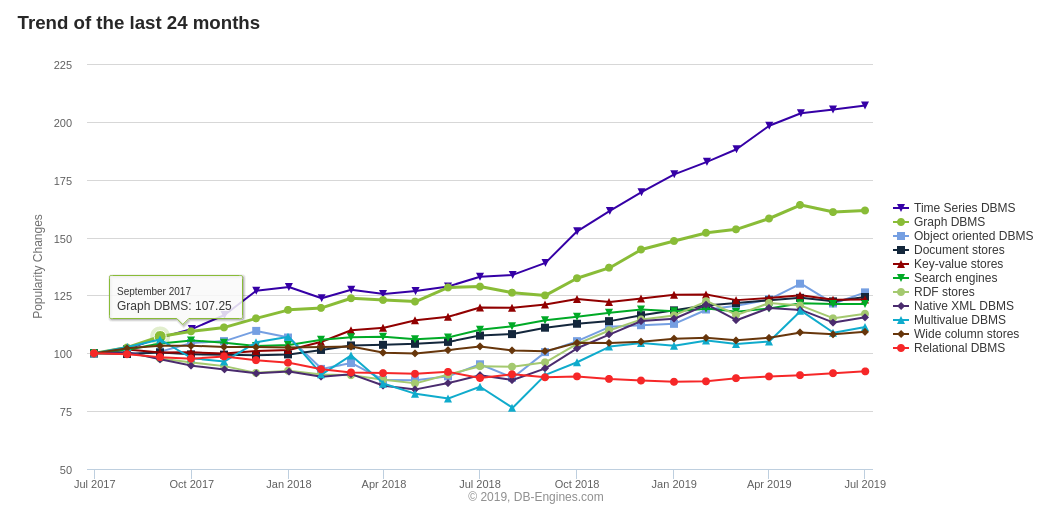
\includegraphics[width=400pt]{tspopularity}
\caption[tspopularity]{Database popularity in the period 2017-2019 according to
\url{https://db-engines.com}, July 2019}
\label{tspopularity}
\end{center}
\end{figure}

Many different businesses rely on the collection and the analysis of this type of data.
DevOps monitoring, scientific measurements, financial markets are just a few business sectors
heavily using time series data.  In most of the applications relying on time series data, it
is vital to collect values as often as possible, to create faster and more accurate monitoring
systems, better models and simulations, more accurate forecasting predictions. As an example,
consider a system that monitors the overall CPU usage of a distributed system. Whenever the
CPU usage exceeds a certain threshold, a remediation action is triggered (for example spawning
an additional node to reduce the load on the system). It is apparent that the usefulness of
the system depends on how often the CPU usage values are collected (the more frequently values are collected, the faster the detection of some anomaly and the faster the remediation action can take place).

The need for finer temporal resolutions requires automatically storing larger quantities of
data, up to the point where traditional relational database systems are not able to handle
the scale. This is because relational database systems store data as a collection of
fixed-size pages on disk. Data is usually indexed by data structures that minimize disk
access, most commonly B-trees. When data sets become large to the point it is not possible
to store indexes in memory anymore, inserting or updating a row might require swapping index
pages from memory to disk, which drastically decreases performance
\cite{Freedman2017Timeseries}. For this reason, new databases that specifically target
time series data have been created. These databases have higher ingestion rates, faster
queries at scale and better data compression as compared to traditional RDBMS. In this
dissertation, I will analyze the problem of data compression in time series data.

\section{Why compressing time series?}
Finding a good compression algorithm to store time series can have multiple benefits depending
on the adopted technique and the use case.
Intuitively, reducing the storage needs of an application allows the system to increase the 
temporal resolution at which the data is recorded.
The storage requirements may be reduced up to the point the whole data set can fit in memory,
reducing writing and reading latency by an order of magnitude or more.
If the application is network bound, compressing data means reducing the amount of data to be
transferred from server to client or the other way around.
In some IoT applications, the compression can be done at the device level, so that less data
need to be transferred over the network. This is usually more power efficient, as the energy
required to compress the data is much less compared to the energy required to transmit it.

\section{Four approaches for time series compression}
We can identify four different approaches for compressing time series data.
\begin{enumerate}
	\item \textbf{Storing aggregates}. In most applications, we are mostly interested in
	recent data as compared to older data. Thus, older data can be $``$aged out$"$ , that is,
	stored in aggregates over a longer temporal interval. Consider the previous example of
	the S\&P Index stock price. Stock prices of the current year can be aggregated over a
	one-hour interval, while older data can be aggregated over days, weeks, and even months.
	One problem with this approach is that aggregates remove fluctuations and outliers that
	are sometimes important when analyzing historical data.
	\item \textbf{Lossless compression}.\ Time series data is characterized by some properties
	that can be exploited to obtain good compression ratios.  For example, most of the time
	data comes at regular intervals, so it does not make sense to store the whole timestamp
	value for each record, but rather go with a delta encoding approach, that is storing only
	the difference between sequential timestamps.
	\item \textbf{Lossy compression. }Many applications are concerned with the trends that
	can be extracted from time series data, and do not require a high level of accuracy. For
	this type of applications, lossy compression can be considered, which usually results in
	much better compression rates as compared to lossless algorithms.
	\item \textbf{General-purpose algorithms}. Some time series databases do not offer
	compression out of the box. In these cases, one can consider running the databases on
	ZFS or other file systems that offer data compression \cite{A2019TimescaleDB}. Other
	benchmarks \cite{Danjou2016Timeseries} have indicated that general-purpose algorithms
	such as LZ4, achieve good compression ratios and may be more desirable to custom solutions
	given their highly efficient implementations.
\end{enumerate}
%!TEX TS-program = pdflatex
%!TEX root = tesi.tex
%!TEX encoding = UTF-8 Unicode

\chapter{Compression techniques for time series data}
  
\chapter{Approaches to Time Series compression}
\section{Storing aggregates}
Storing aggregates is probably the most common approach to deal with large time series.
The idea is to reduce the temporal resolution of data by storing aggregates of values within
some predefined time buckets. Once values have been aggregated to a lower temporal resolution,
they can be deleted, provided that the initial temporal resolution is not needed anymore.
As a practical example, let us consider an application in which we record the time delays
accumulated by trains. The following series represent the daily delay of a specific train on
a certain day in minutes.
\begin{table}[!htbp]
\centering
\begin{tabular}{l|l|l|l|l|l|l}
\textbf{Day 1} & \textbf{Day 2} & \textbf{Day 3} & \textbf{Day 4} & \textbf{Day 5} & \textbf{Day 6} & \textbf{Day 7} \\
\hline
20 & 20 & 10 & 50 & 40 & 40 & 30 \\                
\end{tabular}
\caption{Daily delay of a specific train of a certain day in minutes.}
\label{tab:daily_delay}
\end{table}

After each week passes, we want to aggregate the previous week’s daily data. With reference
to our example above, we can delete the daily values and replace them by their sum
(210 minutes). By also storing the count, we can compute the average daily during that week
(210 / 7 = 30 minutes).
This technique, often called downsampling, is so simple and effective that most time series
databases offer it out of the box. For example, OpenTSDB, an open-source time series database,
offers the possibility to query downsampled data \cite{A2019Downsample}. This is useful when
one wants to plot data keeping the density at a level that can be easily understandable by
users. Admittedly, this feature does not hold any savings in terms of storage, as it is
performed only at query time, but it is still interesting for network bound applications.
Since version 2.4 OpenTSDB offers the possibility to store the result of the downsampler
\cite{A2019Rollup}. In this way, when querying for a long time span, there is no need to wait for the
downsampled data to be computed.
InfluxDB, another popular open-source database, offers the possibility to downsample old
data using continuous queries and retention policy \cite{A2016Downsampling}. Continuous queries
are queries that are run automatically and periodically within a database. Retention policy
defines for how long InfluxDB keeps the data. By using these concepts together, one can use
a continuous query to aggregate old data into a lower temporal resolution and delete the
original data automatically by setting an appropriate retention policy.

\section{Lossless compression}
Lossless compression is a method of data compression that allows to reconstruct the original
data from the compressed data \cite{WikipediaContributors2019Data}. When applied to time series, it is used when we are
interested in retaining the original data but we want to reduce storage space. In this
section, we will present two different algorithms that have been devised to solve different
problems. The first algorithm was created at Facebook to face the huge amount of data
gathered by monitoring their systems. This algorithm has allowed them to store all data
in memory, thus improving considerably reading and writing performance.
The second algorithm we present, called Sprintz, was created to limit the energy consumption
of IoT devices. By sending compressed data, the network interface use is reduced, thus
obtaining considerable power savings.

\subsection{Gorilla}
Gorilla is an in-memory time series database used by Facebook for monitoring the health of
their systems. It was initially presented in a 2015 paper, and it is now available as
open-source software under the name of Beringei \cite{beringei}. Gorilla schema is a simple tuple
composed of three values: the key of the time series stored as a string, the timestamp of the
measurement stored as an integer, and the value stored as a double. 
The compression is applied both to the timestamp and the actual double values. For the
timestamp the delta-of-delta technique is used (which we discussed in chapter 2), while for
the double values a special kind of XOR compression is applied.

\subsubsection{Timestamp compression}
Timestamp compression is achieved by storing the delta of deltas (see previous chapter)
together with a variable-length code.
The algorithm can be described as follows:
\begin{enumerate}
    \item in the block header, we store the initial timestamp $t-1$ which is aligned to a
    two-hour window. The first timestamp $t_0$ is stored as a 14-bit delta from $t-1$.
    \item For the subsequent timestamp $t_n$:
        \begin{enumerate}
            \item calculate the delta of delta $D = (t_n - t_{n-1}) - (t_{n-1} - t_{n-2})$
            \item if delta is 0, store ‘0’
            \item if delta is between [-64, 64], store ‘10’ following the 7-bit value of the
            delta
            \item if delta is between [-256, 256], store ‘110’ following with the 9-bit
            value of the delta
            \item if delta is between [-2048, 2048], store ‘1110’ following the 12-bit value
            of the delta
            \item otherwise, store ‘1111’ followed by the 32-bit value
        \end{enumerate}
\end{enumerate}
This type of compression applied to Facebook experimental data was able to achieve a 96\%
compression ratio. Figure~\ref{gorilla_timestamp} shows the result of the timestamp
compression achieved by Gorilla with Facebook’s data. It is interesting to note that
96\% of the time timestamps were compressed in one bit.

\begin{figure}[]
\begin{center}
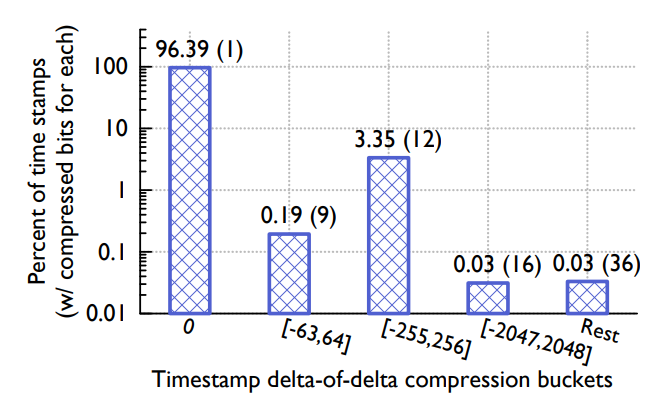
\includegraphics[width=300pt]{gorillaTimestamp}
\caption[gorilla_timestamp]{ Distribution of timestamp compression across different ranged buckets.
Taken from a sample of 440,000 real timestamps in Gorilla \cite{Pelkonen:2015}}
\label{gorilla_timestamp}
\end{center}
\end{figure}

\subsubsection{Compressing values}
Gorilla restricts the value element in its tuple to a double floating-point type. To compress
the values, XOR compression is used together with a variable-length code.
Since values that are close together do not differ by a large amount, the sign, exponent and
few bits of the mantissa are usually the same. Gorilla exploits this by computing the XOR of
the current and previous values. We XOR’d values are then encoded using the following encoding
scheme:
\begin{enumerate}
    \item the first value is stored with no compression
    \item if the XOR with the previous value is 0, then store ‘0’
    \item when XOR is non-zero, calculate the number of leading and trailing zeros in the XOR,
    store bit ‘1’ followed by either a) or b):
        \begin{enumerate}
            \item (control bit ‘0’) If the block of meaningful bits falls within the block of
            previous meaningful bits, i.e., there are at least as many leading zeros and as many
            trailing zeros as with the previous value, use that information for the block position
            and just store the meaningful XORed value
            \item (control bit ‘1’) Store the length of the number of leading zeros in the next
            5 bits, then store the length of the meaningful XORed value in the next 6 bits.
            Finally, store the meaningful bits of the XORed value
        \end{enumerate}
\end{enumerate}
We show an example of this coding in Table~\ref{tab:gorilla}.

\begin{table}[]
\centering
\begin{tabular}{p{1.5cm}|p{3.75cm}|p{4cm}|p{3.5cm}}
\textbf{Decimal} & \textbf{Double \newline representation} & \textbf{XOR with \newline previous} & \textbf{Encoded value} \\ 
\hline
20.5  & 0x4034800000000000 & -                  & 0b010000000011010 \newline 01000000000000000 \newline 00000000000000000 \newline 000000000000000 \\
18    & 0x4032000000000000 & 0x0006800000000000 & 0b110001100000010 \newline 1000100 \\ 
21.5  & 0x4035800000000000 & 0x0007800000000000 & 0b101001110                    \\              
21    & 0x4035000000000000 & 0x0000800000000000 & 0b101000                    \\           
21.25 & 0x4035400000000000 & 0x0000C00000000000 & 0b101100                    \\            
21.25 & 0x4035400000000000 & 0x0000000000000000 & 0b0                    \\            
\end{tabular}
\caption{An example of Gorilla's value compression.}
\label{tab:gorilla}
\end{table}

Using their data set, the authors of Gorilla noted that 51\% of the time subsequent values do
not change at all so they can be stored with one bit (case 2), while 30\% of the time they
have as much leading and trailing zeroes as the previous XOR’d value (case 3a), while the
remaining 19\% are stored with the ‘11’ prefix (case 3b), with an average size of 36.9 bits
due to the 13 bits extra overhead.

\subsection{Sprintz}
Sprintz is a compression algorithm that is specifically tailored for Internet of Things (IoT)
devices \cite{blalock2018sprintz}. These devices have low power consumption and computational limits. Sprintz
reduces the amount of data sent over the network while still being efficient enough to be
run on low powered devices. The design requirements of Sprintz were the following:
\begin{itemize}
    \item \textbf{Small block size}. IoT devices usually do not have much memory, therefore it is not
    possible to buffer large quantities of data. Moreover using large buffers introduces high
    latency which is not favorable for many real-time applications.

    \item \textbf{High decompression speed}. Decompression speed is paramount for all those applications
    which are read-heavy. Compression speed, on the other hand, must only be fast enough to
    keep up with the ingestion rate.
    
    \item \textbf{Lossless}. Instead of assuming that some level of downsampling is appropriate for
    all data, the approach used by Sprintz is to keep the original data quality and leave to
    the developer the choice to downsample data in the preprocessing stage.
\end{itemize}
Sprintz is also targeted to multivariate time series. In a multivariate time series,
each record consists of multiple values. Each value is associated with a dimension. This
contrasts with univariate time series, whereby there is only one dimension.

\subsubsection{Sprintz components}
Sprintz can be described as a bit packing-based predictive coder \cite{blalock2018sprintz}.
It consists of four components:
\begin{itemize}
    \item An online forecaster, that predict the next value in the time series. Sprintz
    saves the error between the predicted value and the real value. This value is supposed
    to be 0 most of the time
    \item A bit packer, that packs the error as a payload and adds sufficient information
    to the header to invert the bit packing
    \item Run-length encoding: Sprintz stores the number of 0 blocks instead of an empty
    payload
    \item Entropy coding: Sprintz uses Huffman coding for the header and the payload
\end{itemize}

\subsubsection{Encoding}
The basic algorithm is outlined in the following pseudo-code listing:

\begin{algorithm}[]
\caption{Sprintz encoding algorithm \cite{blalock2018sprintz}}\label{sprintz_encoding}
\begin{algorithmic}[1]
\Procedure{encodeBlock}{$\{x_1, \ldots, x_b\}$, forecaster}
\State{Let buff be a temporary buffer}
\For {$i \leftarrow 1,\ldots,B$}\Comment{for each sample} \label{line:bodyStart}
    \State{$ \hat{x_i} \leftarrow $ forecaster.predict$(x_{i-1})$}
    \State{$err_i \leftarrow $ $x_i - \hat{x_i}$}
    \State{forecaster.train($x_{i-1}, x_i, err_i$)}
\EndFor
\For {$j \leftarrow 1,\ldots,D$}\Comment{for each column}
    \State{$ nbits_j \leftarrow $ $max_i$\{requiredNumBits$(err_{ij}))$\}}
    \State{$ packed_j \leftarrow $ bitPack($\{err_{1j}, \ldots, err_{Bj}\}, nbits_j$)} 
\EndFor \label{line:bodyEnd}
\State{// Run-length encode if all errors are zero}
\If{$nbits_j$ == $0$, $1 \le j \le D$}
    \Repeat  \Comment{Scan until end of run}
        \State{Read in another block and run lines \ref{line:bodyStart}-\ref{line:bodyEnd}}
    \Until {$\exists_j[nbits_j \neq 0] $}
    
    \State{Write $D$ 0s as headers into buff}
    \State{Write number of all-zero blocks as payload into buff}
    \State{Output huffmanCode(buff)}
\EndIf
\State{Write $nbits_j$, $j = 1,\ldots,D$ as headers into buff}
\State{Write $packed_j$, $j = 1,\ldots,D$ as payload into buff}
\State{Output huffmanCode(buff)}
\EndProcedure
\end{algorithmic}
\end{algorithm}

In line 3-7 the forecaster is used to predict the value, get the error of the forecaster,
and update the forecaster with the current parameters. Then in line 8-11, the maximum number
of bits needed for representing the max value is computed for each column. If all the
dimensions had a 0 error, new blocks are read until an error is found.
Run-length encoding is then used to encode the 0 errors (line 17-19). The header is written
as zeros repeated for the number of dimensions. The payload consists of the number of zero
blocks found. Header and payload are then further compressed using Huffman code. 
If non-zeroes errors were found, then the header will include a header containing the bit
width of each dimension. The values are then packed in the payload. Header and payload are
then encoded using Huffman encoding.

\subsubsection{Decoding}
The decoding is simpler than the encoding. The first step is to decode the Huffman-bitstream
into a header and a payload. Once decoded, the header is examined. If it contains all 0, it
means that the payload was run-length encoded. The number of run-length encoded blocks is
read, and each value can be reconstructed by predicting its value with the forecaster.
If the header does not contain all zeros, then after predicting the value we also need to add
the error value, which is present in the payload. The value will be the predicted value plus
the error value. The forecaster is then updated with the current parameters.

\begin{algorithm}[]
\caption{Sprintz decoding algorithm \cite{blalock2018sprintz}}\label{sprintz_decoding}
\begin{algorithmic}[1]
\Procedure{decodeBlock}{bytes, $B, D$, forecaster}
\State{nbits, payload $ \leftarrow $ huffmanDecode(bytes, $B$, $D$) }
\If{$nbits_j == 0$ $ \forall j $}
    \State{numblocks $ \leftarrow$ readRunLength}
    \For {$i \leftarrow 1,\ldots,(B \times numblocks)$}
        \State{$ x_i \leftarrow $ forecaster.predict$(x_{i-1})$}
        \State{Output $x_i$}
    \EndFor
\Else
    \For {$i \leftarrow 1,\ldots,B$}
        \State{$ x_i \leftarrow $ forecaster.predict$(x_{i-1})$}
        \State{$ err_i \leftarrow $ unpackErrorVector($i$, nbits, payload)}
        \State{$ x_i \leftarrow $ $err_j + \hat{x_i}$}
        \State{Output $x_i$}
        \State{forecaster.train($x_{i-1}, x_i, err_i$)}
    \EndFor
\EndIf
\EndProcedure
\end{algorithmic}
\end{algorithm}

\subsubsection{The forecaster}
Sprintz uses a novel forecaster algorithm called FIRE (Fast Integer REgression). It is
slightly slower than delta encoding but yields a better compression ratio most of the time
\cite{blalock2018sprintz}. Each value is thought of as a linear combination of a fixed amount
of previous values plus some error. The details of the forecaster are outside the scope of
this thesis, but the interested reader can find more in the original paper
\cite{blalock2018sprintz}.

\subsubsection{Bit packing}
Explaining bit packing will be easier by using a practical example. Suppose we want to encode
the following time series:
\begin{table}[!htbp]
\centering
\begin{tabular}{l|l|l}
\textbf{X} & \textbf{Y} & \textbf{Z} \\ 
\hline
5  & 2 & 104 \\
10 & 2 & 103 \\
15 & 2 & 102 \\
20 & 2 & 101 \\
\end{tabular}
\end{table}

We first need to compute the delta. Supposing that the data point immediately preceding
this series was time = -3, value 1 = 2, value 2 = 104, then the delta will look like the
following table:
\begin{table}[!htbp]
\centering
\begin{tabular}{l|l|l}
\textbf{dX} & \textbf{dY} & \textbf{dZ} \\ 
\hline
8 & 0 &  0 \\
5 & 0 & -1 \\
5 & 0 & -1 \\
5 & 0 & -1 \\
\end{tabular}
\end{table}

The next step is to apply the Zigzag encoding. Zigzag encoding is used to transform all
values in nonnegative by representing each integer by twice its absolute value, or twice
its absolute value minus one for negative integers so that positive integers are encoded
as even numbers and negative integers as odd numbers, effectively using the least significant
bit to represent the sign.
\begin{table}[!htbp]
\centering
\begin{tabular}{l|l|l}
\textbf{dX} & \textbf{dY} & \textbf{dZ} \\ 
\hline
16 & 0 &  0 \\
10 & 0 &  1 \\
10 & 0 &  1 \\
10 & 0 &  1 \\
\end{tabular}
\end{table}

The next step is to find the bit width for each column. To do so, for each value we need to
compute the current bit width minus the number of leading zeros. For each column, we take
the maximum of this value, which we will call w. For example, assuming we are 8-bit integers,
16 is represented in binary as $00010000$, so we will have $8 - 3 = 5$ bits necessary to represent
this number. 10 is represented as $00001010$ and requires only 4 bits to be represented.
Therefore we take the max of the two values, 5. The reason why Zigzag encoding was used is
that computing the number of leading zeros can be done in a single assembly instruction
(on systems that support it, such instruction is usually called \texttt{clz}). In the following table
we list the maximum number of bits required to represent each number in each column.
\begin{table}[!htbp]
\centering
\begin{tabular}{l|l|l}
\textbf{dX} & \textbf{dY} & \textbf{dZ} \\ 
\hline
5 & 0 & 1 \\
\end{tabular}
\end{table}

The final step will be to write the header and bit pack the deltas in the payload.
The header will consist of $D$ unsigned integers, one for each column, storing the bit widths.
Each integer in the header is stored in $\log_2{w}$ bits.
In the payload, values are stored contiguously.
In the following table, we use different colors for different columns. Orange will be used
for the $X$ column, green for the $Y$ column and blue for the $Z$ column.

\begin{table}[!htbp]
\centering
\begin{tabular}{l|l|l}
\textbf{Header} & \textbf{Align} & \textbf{Payload} \\ 
\hline
\textcolor{orange}{$101$} \textcolor{green}{$000$} \textcolor{blue}{$001$} & $0000000$ & \textcolor{orange}{$10000$ $01010$ $01010$ $01010$} \textcolor{blue}{$0111$} \\
\end{tabular}
\end{table}

When there are many columns, the bits for each sample are stored contiguously, adding up to
7 bits padding when the sample does not span a multiple of a byte. The reason why this is
not done when there are few columns is that having a 7-bit padding can reduce drastically
the compression ratio, and in the case of univariate data it leads to expansion.

\subsubsection{Entropy coding}
For entropy coding, a Huffman coder is used. This step is optional, but the authors have
observed increased compression ratios using it. Huffman coding is applied after bit packing
for two reasons:
\begin{enumerate}
    \item Reducing the input to the Huffman coding also reduces its latency. This is
    important as Huffman coding is slower than the rest of Sprintz
    \item A better compression ratio is achieved as compared to the case in which Huffman
    coding is applied first.
\end{enumerate}

\section{Lossy compression algorithms}
This family of algorithms uses inexact approximations to represent a data series. In
contrast with lossless compression, these algorithms do not allow to compress data and
keep the full resolution of it. In this section, we will present some algorithms that use
this approach. A feature of the algorithms that we present is that they allow for quality
guarantees to be defined, that is, users can define how much the compressed values can differ
from the original value. In the following sections, we will analyze Piecewise Constant
Approximation, Piecewise Linear Approximation, and ModelarDB, a time series database that
makes use of multiple algorithms to optimize the compression ratio based on the user-defined
quality guarantees.

\subsection{Piecewise Constant Approximation}
Piecewise constant approximation represents a time series S as a sequence of K segments
\cite{keogh2001locally}\cite{lazaridis2003capturing}:
$$PCA(S^n) = \langle(c_1, e_1), (c_2, e_2), \ldots, (c_k, e_k))\rangle$$
where $e_k$  is the end-point of a segment and $c_k$ is a constant value for time in
$[e_{k-1} + 1, e_k]$ or for time in $[1, e_1]$ for the first segment. If each segment
corresponds to many samples of the series, then high compression ratios can be achieved.
In \cite{lazaridis2003capturing}, a simple algorithm name Poor Man’s Compression -
Midrange (PMC-MR) was proposed to construct a PCA  representation of a series with
$O(1)$ space requirements and $O(n)$ time complexity, where $n$ is the number of samples
in a series. This algorithm does also take into consideration quality guarantees, that
is, users can decide the maximum acceptable quality loss the algorithm will produce.
Algorithm~\ref{PMC_MR} lists the procedure taken from \cite{lazaridis2003capturing}.

\begin{algorithm}
\caption{Poor Man's Compression Midrange \cite{lazaridis2003capturing}}\label{PMC_MR}
\begin{algorithmic}[1]
\Procedure{pcr}{series, tolerance}
\State{PCA(series) $ \leftarrow $ $\langle \rangle$ }
\State{n $ \leftarrow $ $1$ }
\State{m $ \leftarrow $ series[n] }
\State{M $ \leftarrow $ series[n] }
\While{series.hasMoreSamples()}
    \If{max\{M, series[n]\} - min\{m, series[n]\} $>$ 2 x tolerance}
        \State{\textbf{append}($\frac{M + m}{2}, n-1$) \textbf{to} PCA(series)}
        \State{m $ \leftarrow $ series[n] }
        \State{M $ \leftarrow $ series[n] }
    \Else
        \State{m $ \leftarrow $ min\{m, series[n]\} }
        \State{M $ \leftarrow $ max\{M, series[n]\}}
    \EndIf
    \State{n $ \leftarrow $ n + 1 }
\EndWhile
\State{\textbf{append}($\frac{M + m}{2}, n-1$) \textbf{to} PCA(series)}
\State{\textbf{return} PCA(series)}
\EndProcedure
\end{algorithmic}
\end{algorithm}

The procedure uses $n$ to represent the endpoint of the segment, and represents the
minimum and maximum values found in the segment not yet pushed to the PCA with $m$ and
$M$. In each cycle, we evaluate whether the range we are considering is no more than
twice the quality boundary. If that is the case, we update $m$ and $N$. Once the current
range exceeds this quality boundary, we push $\frac{m + M}{2}$  up until $n - 1$ and we
reset $m$ and $M$ to the current value (which was not included in the current segment).
As a practical example, suppose we have the following series:
$$S = 22, 24, 31, 32, 33, 37$$
If our quality guarantee is 3 (that is, the absolute value of the difference between the
compressed value and the original value should never exceed 3), the series will be
compressed to the following PCA:
$$PCA = \langle(23, 2), (34, 6) \rangle$$
In Figure~\ref{pca} we have a visual representation of how the series has changed.

\begin{figure}[!htbp]
\begin{center}
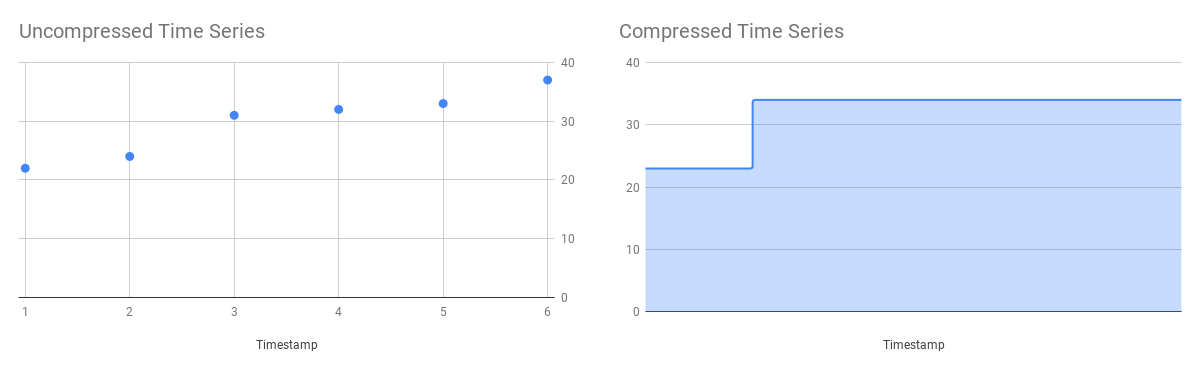
\includegraphics[width=400pt]{pca}
\caption[pca]{A time series before and after applying the PMC-MR algorithm.}
\label{pca}
\end{center}
\end{figure}

\subsection{Piecewise Linear Approximation}
Piecewise Linear Approximation (PLA) is the natural evolution of PCA. Instead of
approximating multiple values with a single constant value, we approximate a time series
S with k straight lines. Algorithm~\ref{PLA} is one popular algorithm that produces a PLA.

\begin{algorithm}
\caption{Online Piecewise Linear Approximation \cite{lazaridis2003capturing}}\label{PLA}
\begin{algorithmic}[1]
\Procedure{pla}{series, tolerance}
\State{PLA(series) $ \leftarrow $ $\langle \rangle$ }
\State{anchor $ \leftarrow $ 1 }
\While{not finished segmenting time series}
    \State{i $ \leftarrow $ 2 }
    \While{calculateError(series[anchor:anchor $+ i$]) $<$ tolerance }
        \State{anchor $\leftarrow$ anchor + 1}
    \EndWhile
    \State{\textbf{append} createSegment(series[anchor:anchor+i]) \textbf{to} PLA(series)}
\EndWhile
\State{\textbf{return} PLA(series)}
\EndProcedure
\end{algorithmic}
\end{algorithm}

This algorithm resembles PMC-MR, in that it grows a segment until it can fit the user-defined
max error. The algorithm keeps track of two variables: anchor, which define the start index
of a potential segment, and $i$, which defines the end of the segment. It appends the generated
segments to PLA, a variable referencing a list.  In line 6-7 it checks
whether the segment from anchor to anchor + $i$ is able to represents the original values
within the tolerance value defined.
When this condition is satisfied, the index $i$ is increased. If that is not the case,
then the segment from anchor to anchor + $i - 1$ is appended to the PLA(series)
and the anchor variable is updated. The approximation can be improved by using other variations.
Most of them are batch algorithms \cite{douglas1973algorithms}\cite{park1999fast}
\cite{keogh1998enhanced}, but some online alternatives have been
proposed as well \cite{keogh2001online}.

\subsection{ModelarDB}
ModelarDB is a time series database management system that was designed to store and query
massive amounts of high-quality sensor data ingested in real-time from many sensors
\cite{jensen2018modelardb}.
To tackle these problems, model-based compression was used. Model-based compression is a
lossy compression technique that stores a representation that can recreate data within a
known error bound. For example, PLA is a type of model-based compression, using linear
equations to represent data. ModelarDB is model agnostic, this means that it uses multiple
models depending on the one with the best fit. It also supports user-defined models.
Users can extend the system with their own compression models.

\subsubsection{Model-Agnostic Compression Algorithm}
ModelarDB uses a model agnostic compression algorithm so that users can extend the set of
compression models. Data is stored as segments, where each segment stores multiple data
points and can use a different model. In order to satisfy latency constraints, two types
of segments are used, namely a temporary segment (ST) and a finalized segment (SF).
The STs are emitted based on a user-defined latency in terms of data points not yet
emitted to the stream, while SFs are emitted when a new data point cannot be represented
by the set of models used.
We have an example of how the algorithm works in Figure~\ref{modelar}. For this example,
the latency is three data points, and a single linear model is used. At $t_3$  we have three
points, and an ST is emitted since the number of represented points equals the latency.
As the model M might be able to fit more data points, the points are kept in a buffer and
the next data point is added at $t_4$. At $t_5$, M cannot fit all data points within the
user-specified error bound, so it emits then an SF with the 4 fittable values and a
new segment is created from datapoint 5. After a user-defined bulk write size is
reached,  the segments are flushed to disk.
The pseudo-code is listed in Algorithm~\ref{alg_modelar}.
\begin{figure}
\begin{center}
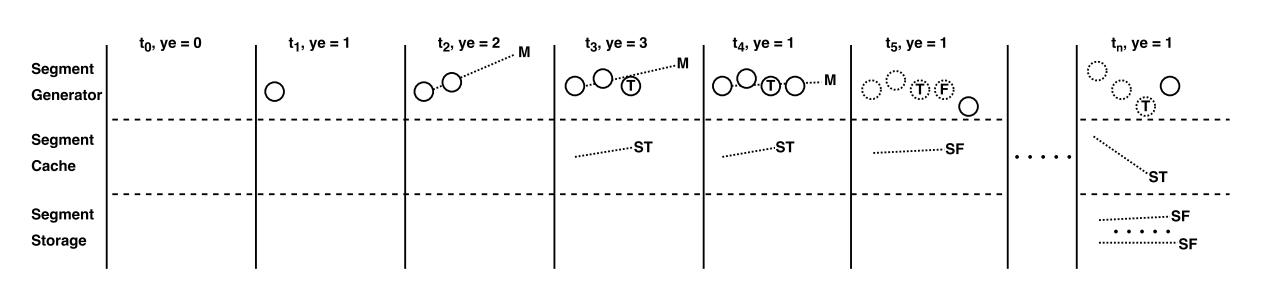
\includegraphics[width=400pt]{modelar}
\caption[modelar]{A depiction of the ModelarDB compression algorithm, taken from \cite{jensen2018modelardb}}
\label{modelar}
\end{center}
\end{figure}
\begin{algorithm}
\caption{Online model-agnostic compression algorithm \cite{jensen2018modelardb}}\label{alg_modelar}
\begin{algorithmic}[1]
\Procedure{modelarDB}{series, tolerance}
\State{Let series be the time series of data points}
\State{Let models be the list of models to select from}
\State{Let tolerance be the user defined error bound}
\State{Let limit be the limit on the length of each segment}
\State{Let latency be the latency in non emitted data points}
\State{Let interval be the sampling interval of the time series}

\State{model $ \leftarrow $ models.head() }
\State{buffer $ \leftarrow $ createList()}
\State{yetEmitted $ \leftarrow $ $0$}
\State{previous $ \leftarrow $ $nil$}

\While{series.hasMoreSamples()}
    \State{dataPoint = series.getNextDataPoint()}
    \If{timeDifference(previous, dataPoint) $>$ interval}
        \State{flushBuffer(buffer)}
    \EndIf
    \State{appendDataPointToBuffer(dataPoint, buffer)}
    \State{previous $\leftarrow$ dataPoint}
    \If{appendDataPointToBuffer(\par
        \hskip\algorithmicindent dataPoint, buffer, tolerance, limit)}
        \State{yetEmitted $\leftarrow$ yetEmitted + 1}
        \If{yetEmitted = latency}
            \State{emitTemporarySegment(model, buffer)}
            \State{yetEmitted $\leftarrow$ 0}
        \EndIf
    \ElsIf{models.hasMoreModels()}
        \State{model $\leftarrow$ models.getNextModel()}
        \State{initialize(model, buffer)}
    \Else
        \State{emitFinalizedSegment(models, buffer)}
        \State{model $\leftarrow$ models.head()}
        \State{initialize(model, buffer)}
        \State{yetEmitted $\leftarrow$ min(yetEmitted, buffer.length())}
    \EndIf
\EndWhile
\State{flushBuffer(buffer)}
\EndProcedure
\end{algorithmic}
\end{algorithm}
After initializing variables, we iterate through all the values of the time series (line 12).
In case a value was lost, we flush the current buffer (lines 14-16). The data point is then
added to the buffer, and we set previous to the current data point. The data point is then
added to the model. If the model can still fit the data point, the yetEmitted variable is
increased. If this variable has reached the user-defined latency, then a temporary segment
is emitted and the variable is set to 0.
If the model cannot accept another data point without exceeding the user-defined error,
then a new model is initialized with the current buffer (lines 25-27). When the list of
models becomes empty, an SF containing the model with the highest compression ratio is
emitted in line 29. We then initialize the first model with the remaining points in the
buffer (lines 30-31).
In line 32 we update yetEmitted to reflect the decrease in the number of emitted points.
Finally, we flush the remaining data points in the buffer in line 35.

\section{General-purpose algorithms}
In this section, we will analyze some general-purpose algorithms that have been used in
time series databases. We start with LZ4, an extremely fast compression algorithm inspired
by LZ77. We continue with Deflate, an algorithm that mixes dictionary compression and entropy
compression. We will finish with ZStandard, an open-source Deflate alternative.

\subsection{LZ4}
LZ4 is a lossless compression algorithm focused on compression and decompression speed
based on LZ77 \cite{ziv1977universal}\cite{lz42019lz4lz4}. As LZ77, LZ4 uses a sliding windows
consisting of a search buffer and a look-ahead buffer. Repetitive data is replaced with
an index to the search buffer. An LZ4 compressed block is composed of sequences.
A sequence consists of a token, literal length, offset and matched length, as
shown in the following table.
\begin{table}[!htbp]
\centering
\begin{tabular}{l|l|l|l|l}
\textbf{Token} & \textbf{Literals Length} & \textbf{Literals} & \textbf{Offset} & \textbf{Match Length} \\ 
\hline
1 byte & $0-n$ bytes & $0-|Literals|$ bytes & 2 bytes & $0-n$ bytes \\
\end{tabular}
\end{table}

The token is a 1-byte value separated in two 4 bits fields. The four most significant bits,
which can range from 0 to 15, represent the length of the literals that will follow. Since
the literals can be of any length, bytes are dynamically added if they cannot fit in the 4
bits. For example, suppose we want to represent
the value 470. Then the first part of the token will be set to 15, and we would need to
read a byte from the literal length part. This byte will be 255. When the byte is 255,
we need to read a new byte. This byte will be 200. When the byte is not 255, we know that
this was the last byte in the literal length part. So in total we will have
15 + 255 + 200 = 470 bits.
This mechanism scales linearly with the length of literals, but this usually is not a problem
since most of the time the length of the literal is small.
The four least significant bits of the token indicates the match length. As with the
length of the literal, this number has no limitations and can be expanded by adding new
bytes to the match length section of the block.
Following the token and the length of the optional literal, we have the literals part of
the block. It is possible that this part is skipped (this happens when the word is
entirely matched in the dictionary).
The offset is composed of two bytes, and it represents the offset from the position where
the match begins.
Let us make a practical example. Suppose that during the LZ4 compression we have the following
binary string in our search buffer
$$S = 00001111000011110101$$
We want to compress the following string by refering the search buffer:
$$S' = 0011110000111101011111$$
We notice that the first 18 bits are identical to the last 18 bits in the search buffer. Thus
we will only need to include the last 4 bits in the literals section of the block.
We already know how the token byte will look like: 0100$|$1111. The first 4 bits indicate that
we have a 4 bits literal length. The last 4 bits indicate that we have a match bigger than
15 bits, therefore we need to check for additional bytes in the match length part of the block.
Since the literals length is $< 15$, we do not need any literals length additional bytes.
Next we can encode the literals as 1111. We then need to encode the offset, which is 18.
So far we have the following bits: $01001111 1111 00000000 00010010$.
The last part is to include an additional match length byte, to obtain 18 bits of matched
length. This last byte will encode 3 (we must sum the 15 bits of the token to obtain 18).
The final block encoding $S'$ thus looks like the following:
\begin{table}[!htbp]
\centering
\begin{tabular}{l|l|l|l|l}
\textbf{Token} & \textbf{Literals Length} & \textbf{Literals} & \textbf{Offset} & \textbf{Match Length} \\ 
\hline
01001111 & / & 1111 & 00000000 00010010 & 00000011 \\
\end{tabular}
\end{table}

\subsection{Deflate}
Deflate uses both LZ77 and Huffman coding to achieve compression \cite{LPeterDeutsch1996DEFLATE}. 
A compressed data set is composed of blocks. Each block can use a
different “mode” of compression. There are three available modes:
\begin{enumerate}
    \item No compression. Useful when data has already been compressed
    \item Compression, with LZ77 and Huffman coding in sequence. The trees
    used are the ones in the specification.
    \item Compression, with LZ77 and Huffman coding. The compressor
    creates the trees and store them with the data.
\end{enumerate}
Each block consists of two parts: a pair of Huffman code trees that describe the
representation of the compressed data part, and a compressed data part. The compressed
data parts consist of literals and pointers to the duplicated strings, represented as
$<length, distance>$ pairs. Each type of value (literals, distances and lengths) in the
compressed data is represented using Huffman code, using one code tree for literals and
lengths and a separate one for distances. When using compression mode 2, the Huffman codes
are not explicitly represented in the data, as they can be generated by the decompressor.
This is because mode 2 uses a Huffman tree with two further restrictions as compared to
the standard Huffman tree:
\begin{itemize}
    \item elements with shorter codes are placed left to element with longer codes
    \item elements with the same length are ordered lexicographically
\end{itemize}
The reason why these two restrictions are placed upon trees, is that with these restrictions
for a given set of elements and their respective length there is only one possible tree.
When using mode 3, the Huffman codes for the two alphabets must be included. Deflate has
many implementations that differ in some minor details. The most popular are zip, gzip, and
zlib.

\subsection{ZStandard}
ZStandard was built to be a replacement for deflate for faster and more effective compression
\cite{ColletY2018Smaller}. It uses Finite State Entropy (FSE) \cite{ColletY2013Finite}
and it is optimized for modern CPUs. Finite State Entropy can be seen as a replacement
for Huffman encoding: it allows for the same compression ratio while improving
on the speed \cite{ColletY2013Finite}. The details of FSE are outside the scope of
this thesis, but the interested reader can find more information in \cite{ColletY2013Finite}
\cite{ColletY2014FSE}.
ZStandard is a versatile compression algorithm, suitable for usage in widely
different circumstances. It is faster both in compression and decompression
speed as compared to zlib, while achieving similar compression ratios \cite{ColletY2018Smaller}.
ZStandard offers also a specific training mod, which can be used to tune the algorithm for a selected
type of data. The result of the training is stored in a dictionary which will be loaded before compression
and decompression. This can be an interesting use case for compressing
JSON data returned by web services \cite{ColletY2018Smaller}.

\chapter{Empirical evaluation of compression algorithms}
In this chapter, we compare different compression algorithms in terms of compression ratio using both real
and generated time series data. The compression algorithms that we have chosen are Gorilla, LZ4,
Deflate and Zstandard. By doing this we want to evaluate whether compression algorithms specifically
targeted to time series are better than general-purpose algorithms.

\section{Datasets}
For these benchmarks, we have used three different datasets. The first dataset was generated from the
Time Series Benchmark Suite, a command-line tool written by TimescaleDB \cite{timescale_2019_timescaletsbs} that makes
easy to generate realistic time-series data to benchmark different time series databases.
The second dataset was created by using Dynatrace. Dynatrace is a Software Intelligence platform with a strong
emphasis on application performance monitoring. The datasets consist of metrics gathered from
different hosts running a wide range of applications under different loads.
The third dataset was provided by the New York Taxi and Limousine Commission (TLC), and it consists
of records representing taxi trips, including information such as duration of the trip, amount
charged, tip amount \cite{tlc2019_dataset}.

\subsection{Generating devops data}
As we have mentioned above, we have used the TimeSeries Benchmark Suite to generate fake DevOps data.
This utility allows to specify which use case to simulate data for, which time interval between each data points
to use, the starting timestamp and the ending timestamp, how many hosts to simulate.
We have decided to generate data points every minute, for a single host and for 5 different time intervals:
2 hours, 4 hours, 8 hours, 16 hours and 48 hours. For each of these intervals, we generate 50 different time-series.

\subsection{Collecting Dynatrace Data}
Dynatrace provides a REST API to retrieve metrics it collects \cite{a2013_metrics}.
We have used this API to retrieve data of several hosts which were monitored in one of the demo environment
Dynatrace uses for testing purposes.
The metrics we have chosen to collect are the following:
\begin{itemize}
    \item Host CPU Usage: Percentage of overall CPU usage
    \item Host CPU System: Percentage of CPU time used by the kernel
    \item Host CPU User: Percentage of CPU time used by userspace processes
    \item Host CPU Io Wait: Percentage of CPU time spent waiting for input/output operations
    \item Host Memory Used: Percentage of memory used
    \item Host Memory Usage: Memory usage in bytes
    \item Host Disk Read Time: Disk read time in milliseconds
    \item Host Disk Write Time: Disk write time in milliseconds
\end{itemize}

\subsection{Taxi Data}
The taxi data set was provided by the New York Taxi and Limousine Commission. For each month of the year,
the TLC provide a data set for the two different taxi companies running in New York (green and yellow)
and for limousines. We have decided to take into account only yellow taxi data for one month.
Moreover, to make in-memory compression feasible, we have dropped the last 3 million records from the
dataset. Additionally, all the columns containing string data were removed since they are not handled
by the Gorilla algorithm.

\section{Compressing data}
The metric which we are interested in these benchmarks is the compression ratio, while we do not evaluate compression speed
as this is dependent on the specifics algorithms implementations.
We have created a Java program that reads data from the input stream and returns the compression ratio
achieved by the algorithm selected. We decided to use Java because we could easily find implementations for
all the algorithms listed above.
The program requires to specify the format of the dataset provided in the standard input and the
algorithm to use for compression, as the following listing illustrates.
\lstset{
    basicstyle=\small,
    stringstyle=\ttfamily
}
\begin{lstlisting}[language=bash]
  $ ./gradlew shadowJar
  $ java -jar
  TimeseriesCompressionBenchmarks-all.jar [format] [algorithm]
\end{lstlisting}
Gorilla compression does not work on byte data. It needs instead pairs of values and timestamps.
For this reason, we parse each time-series file to obtain a TimeSeries object.
This object contains a key and a list of value-timestamp pairs.  
We pass this TimeSeries object to a compressor, which is an interface responsible for returning a compressed version of the time-series.
In the case of Gorilla compression, we have implemented this interface by iterating through all
the data points, pushing those to the Gorilla compression library, and returning the compressed
version of the time-series, which is a long array in the case of the Gorilla Compression library we are using.
With the other compression algorithms, we could serialize the TimeSeries
object to a byte array, compress it, and get back a compressed byte array. 
The way we compute the compression ratio is by dividing the number of bytes representing the serialized
time-series object, divided by the number of bytes of the serialized compressed time-series.
The code is available on github \cite{dovidio_2019_dovidiotscompressionthesis}.
For gorilla compression, we have used an open source java implementation of the algorithm
\cite{burmanm_2018_burmanmgorillatsc}. Deflate, on the other hand, is already present in the the package
\textit{java.util.zip}, using the zlib library under the hood \cite{a2019_deflater}.
For LZ4 and ZStandard we have used open source implementations \cite{lz4_2019_lz4lz4java}\cite{luben_2015_lubenzstdjni}.

\section{Results}
\subsection{Generated data}
Figure~\ref{devops_lossless_compression} illustrates the result of applying different compression algorithms
with generated data. It clearly shows how Gorilla (mean = 13.35, standard deviation = 1.60), is outperforming the other
lossless compression algorithms.
It is also interesting to notice how ZStandard (mean = 3.58, standard deviation = 0.32) and Deflate
(mean = 3.22, standard deviation = 0.24)
performs similarly, while LZ4 (mean = 2.36, standard deviation = 0.14) has
consistently the worst compression ratio, as one might have predicted given that it was engineered to optimize compression speed rather
than compression ratio.

\begin{figure}[!htbp]
\begin{center}
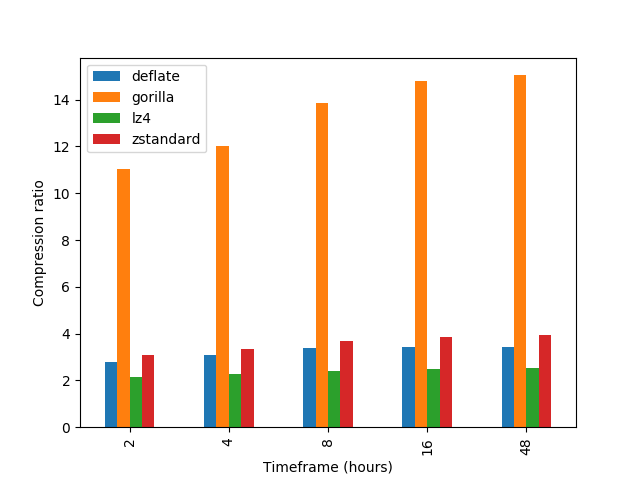
\includegraphics[width=300pt]{devops_bar_chart}
\caption[compression]{Generated data compressed with Gorilla, Deflate, ZStandard, LZ4.
Higher values indicates higher compression ratios.}
\label{devops_lossless_compression}
\end{center}
\end{figure}

\subsection{Dynatrace Data}
Results of the different compression algorithms applied to real-word series data are shown in
Figure~\ref{dynatrace_compression}. The results are similar to what we have seen for generated data,
with Gorilla (mean = 3.40, standard deviation = 0.10) outperforming all the other general purposes algorithm across all metrics.
As we also saw in the previous benchmark, deflate (mean = 2.16, standard deviation = 0.34) and zstandard (mean = 2.15, standard deviation = 0.42)
have a similar performance, which is significantly better than LZ4 (mean = 1.77, standard deviation = 0.19).
It is interesting to notice that although Gorilla provides the best compression here, it is much lower as compared to the compression achieved with generated data.
By having a closer look at both sources of data, we hypothesized that this is because the generated data contains repeated consecutive values
much more often as compared to real-world data. Gorilla is optimized to reduce the storage need for this particular case, and this
alone would explain the big difference.
Indeed a closer inspection reveals that the percentage of repeated values in the case of generated data is $41\%$, while in the case
of real-world data is $0.76\%$.
This happens because most values were generated using a random walk distribution which results in a high correlation between the values. Moreover, most of the generated
values are integers. One interesting thing we have also noted is that the time series benchmark tool is that it tends to create more values when the timeframe is larger.
When it comes to data gathered by Dynatrace, all the values are represented as floating-point values. Although the delta between the values tend to be small most of
the time, the chances of getting the same value in a sequence are much smaller with high-resolution real data.  

\begin{figure}[!htbp]
\begin{center}
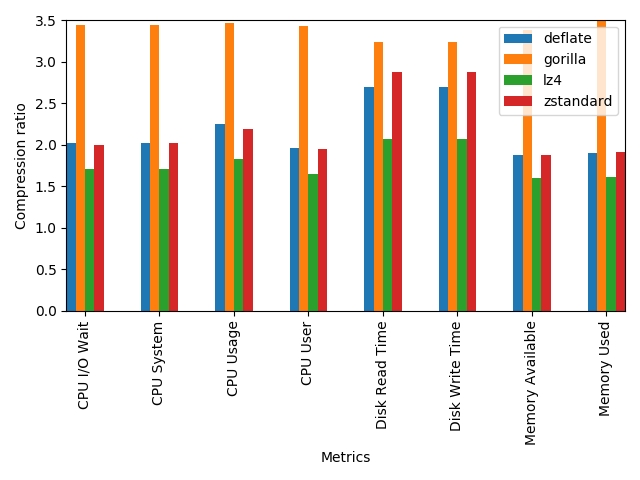
\includegraphics[width=300pt]{dynatrace_bar_chart}
\caption[compression]{Real world data collected by Dynatrace compressed with Gorilla, Deflate, ZStandard, LZ4.
Higher values indicates higher compression ratios.}
\label{dynatrace_compression}
\end{center}
\end{figure}

\subsection{Taxi Data}
For taxi data, we have decided to transform the data in a column format.
Since each record contains 15 columns, this means that we have transformed data in 15 time series,
ordered by pick up time.
Each time series data point represent a specific value for a specific taxi trip.
The time interval between each data point is not regular as in the previous data sets, for this
reason Gorilla delta of delta timestamp compression is likely to not yield good compression
ratios. Moreover since there is no correlation between taxi trips, XOR compression of float will
not be effective.
Having a look at the results in Figure~\ref{taxi_bar_chart}, we can see that indeed Gorilla compression does not perform well as
in the other benchmarks. The best compression algorithms in this case are deflate (achieving a compression
ratio of 6.78) and zstandard (achieving a compression ratio of 6.70). Gorilla performs slightly
better than LZ4 (4.80 vs 4.11).

\begin{figure}[!htbp]
\begin{center}
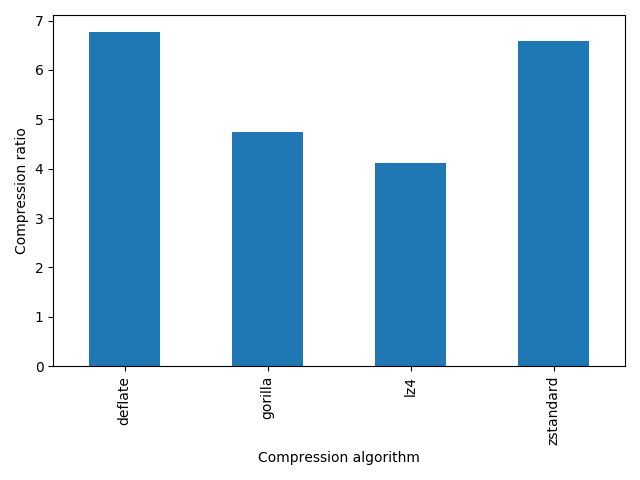
\includegraphics[width=300pt]{taxi_bar_chart}
\caption[compression]{Taxi Data compressed with Gorilla, Deflate, ZStandard, LZ4.
Higher values indicates higher compression ratios.}
\label{taxi_bar_chart}
\end{center}
\end{figure}

\subsection{Discussion}
From our limited results, it is hard to say which compression algorithm is the best for time-series data.
Although Gorilla seems to allow for greater compression ratios for DevOps data, this is not the case when
time-series data has no correlation, and when the interval between data points is irregular.
Deflate and ZStandard offers good compression ratios and they have the advantage to have many stable and
optimized implementations.
LZ4 performed consistently worse than the other algorithms in each of the benchmarks, but might be chosen
for those applications where compression and decompression speed are important.


\chapter*{Conclusions}
This thesis aimed to identify the principal approaches and algorithms for time-series data compression.
We have identified four main approaches that are used in real-world applications and databases.
We then created a benchmark to evaluate how Gorilla, an algorithm specifically tailored for infrastructure
monitoring time-series data, performs against state of the art general purposes algorithms. 
These benchmark clearly illustrates how Gorilla can outperform the general purposes algorithm, but it
also shows how this is highly dependent on the correlation between values in the time series.
Based on these results, it is vital to understand the type of data one is dealing with. Our benchmarks
showed that the best results are obtained with time-series data sets whereby the same values are repeated
in neighboring data points. Future research should consider the speed of compression and decompression of
these algorithms. This might be interesting especially when dealing with database queries. On the one hand,
having less data stored might speed up the queries. On the other hand, decompression speed should also
be taken into account.
\addcontentsline{toc}{chapter}{Conclusions}
\appendix

\printbibliography



\backmatter



% \printindex % se si fa l'indice analitico.

\end{document}
